%----------------------------------------------------------------------------------------
%	
%----------------------------------------------------------------------------------------

%----------------------------------------------------------------------------------------
%	CONFIGURACION DOCUMENTO
%----------------------------------------------------------------------------------------

\documentclass{article}

%%%%%%%%%%%%%%%%%%%%%%%%%%%%%%%%%%%%%%%%%
% Lachaise Assignment
% Structure Specification File
% Version 1.0 (26/6/2018)
%
% This template originates from:
% http://www.LaTeXTemplates.com
%
% Authors:
% Marion Lachaise & François Févotte
% Vel (vel@LaTeXTemplates.com)
%
% License:
% CC BY-NC-SA 3.0 (http://creativecommons.org/licenses/by-nc-sa/3.0/)
% 
%%%%%%%%%%%%%%%%%%%%%%%%%%%%%%%%%%%%%%%%%

%----------------------------------------------------------------------------------------
%	IDIOMA
%----------------------------------------------------------------------------------------

\usepackage[spanish]{babel}

%----------------------------------------------------------------------------------------
%	PACKAGES AND OTHER DOCUMENT CONFIGURATIONS
%----------------------------------------------------------------------------------------

\usepackage[table,xcdraw]{xcolor}
\usepackage{booktabs}

\usepackage{multicol}

\usepackage{multirow}

\usepackage{amsmath,amsfonts,stmaryrd,amssymb} % Math packages

\usepackage{enumerate} % Custom item numbers for enumerations

\usepackage[ruled]{algorithm2e} % Algorithms

\usepackage[framemethod=tikz]{mdframed} % Allows defining custom boxed/framed environments

\usepackage{listings} % File listings, with syntax highlighting
\lstset{
	basicstyle=\ttfamily, % Typeset listings in monospace font
}

%----------------------------------------------------------------------------------------
%	DOCUMENT MARGINS
%----------------------------------------------------------------------------------------

\usepackage{geometry} % Required for adjusting page dimensions and margins

\geometry{
	paper=a4paper, % Paper size, change to letterpaper for US letter size
	top=2cm, % Top margin
	bottom=2cm, % Bottom margin
	left=2cm, % Left margin
	right=2cm, % Right margin
	headheight=14.2pt, % Header height
	footskip=1.3cm, % Space from the bottom margin to the baseline of the footer
	headsep=0.8cm, % Space from the top margin to the baseline of the header
	%showframe, % Uncomment to show how the type block is set on the page
}

%----------------------------------------------------------------------------------------
%	FONTS
%----------------------------------------------------------------------------------------

\usepackage[utf8]{inputenc} % Required for inputting international characters
\usepackage[T1]{fontenc} % Output font encoding for international characters

\usepackage{XCharter} % Use the XCharter fonts

%----------------------------------------------------------------------------------------
%	COMMAND LINE ENVIRONMENT
%----------------------------------------------------------------------------------------

% Usage:
% \begin{commandline}
%	\begin{verbatim}
%		$ ls
%		
%		Applications	Desktop	...
%	\end{verbatim}
% \end{commandline}

\mdfdefinestyle{commandline}{
	leftmargin=10pt,
	rightmargin=10pt,
	innerleftmargin=15pt,
	middlelinecolor=black!50!white,
	middlelinewidth=2pt,
	frametitlerule=false,
	backgroundcolor=black!5!white,
	frametitle={Command Line},
	frametitlefont={\normalfont\sffamily\color{white}\hspace{-1em}},
	frametitlebackgroundcolor=black!50!white,
	nobreak,
}

\mdfdefinestyle{commandline2}{
	leftmargin=5pt,
	rightmargin=5pt,
	innerleftmargin=15pt,
	middlelinecolor=black!50!white,
	middlelinewidth=2pt,
	frametitlerule=false,
	backgroundcolor=black!5!white,
	frametitle={Command Line},
	frametitlefont={\normalfont\sffamily\color{white}\hspace{-1em}},
	frametitlebackgroundcolor=black!50!white,
	nobreak,
}
% Define a custom environment for command-line snapshots
\newenvironment{commandline}{
	\medskip
	\begin{mdframed}[style=commandline]
}{
	\end{mdframed}
	\medskip
}

\newenvironment{commandline22}{
	\medskip
	\begin{mdframed}[style=commandline2]
}{
	\end{mdframed}
	\medskip
}

%----------------------------------------------------------------------------------------
%	FILE CONTENTS ENVIRONMENT
%----------------------------------------------------------------------------------------

% Usage:
% \begin{file}[optional filename, defaults to "File"]
%	File contents, for example, with a listings environment
% \end{file}

\mdfdefinestyle{file}{
	innertopmargin=1.6\baselineskip,
	innerbottommargin=0.8\baselineskip,
	topline=false, bottomline=false,
	leftline=false, rightline=false,
	leftmargin=2cm,
	rightmargin=2cm,
	singleextra={%
		\draw[fill=black!10!white](P)++(0,-1.2em)rectangle(P-|O);
		\node[anchor=north west]
		at(P-|O){\ttfamily\mdfilename};
		%
		\def\l{3em}
		\draw(O-|P)++(-\l,0)--++(\l,\l)--(P)--(P-|O)--(O)--cycle;
		\draw(O-|P)++(-\l,0)--++(0,\l)--++(\l,0);
	},
	nobreak,
}

% Define a custom environment for file contents
\newenvironment{file}[1][File]{ % Set the default filename to "File"
	\medskip
	\newcommand{\mdfilename}{#1}
	\begin{mdframed}[style=file]
}{
	\end{mdframed}
	\medskip
}

%----------------------------------------------------------------------------------------
%	NUMBERED QUESTIONS ENVIRONMENT
%----------------------------------------------------------------------------------------

% Usage:
% \begin{question}[optional title]
%	Question contents
% \end{question}

\mdfdefinestyle{question}{
	innertopmargin=1.2\baselineskip,
	innerbottommargin=0.8\baselineskip,
	roundcorner=5pt,
	nobreak,
	singleextra={%
		\draw(P-|O)node[xshift=1em,anchor=west,fill=white,draw,rounded corners=5pt]{%
		Question \theQuestion\questionTitle};
	},
}

\newcounter{Question} % Stores the current question number that gets iterated with each new question

% Define a custom environment for numbered questions
\newenvironment{question}[1][\unskip]{
	\bigskip
	\stepcounter{Question}
	\newcommand{\questionTitle}{~#1}
	\begin{mdframed}[style=question]
}{
	\end{mdframed}
	\medskip
}

%----------------------------------------------------------------------------------------
%	WARNING TEXT ENVIRONMENT
%----------------------------------------------------------------------------------------

% Usage:
% \begin{warn}[optional title, defaults to "Warning:"]
%	Contents
% \end{warn}

\mdfdefinestyle{warning}{
	topline=false, bottomline=false,
	leftline=false, rightline=false,
	nobreak,
	singleextra={%
		\draw(P-|O)++(-0.5em,0)node(tmp1){};
		\draw(P-|O)++(0.5em,0)node(tmp2){};
		\fill[black,rotate around={45:(P-|O)}](tmp1)rectangle(tmp2);
		\node at(P-|O){\color{white}\scriptsize\bf !};
		\draw[very thick](P-|O)++(0,-1em)--(O);%--(O-|P);
	}
}

% Define a custom environment for warning text
\newenvironment{warn}[1][Warning:]{ % Set the default warning to "Warning:"
	\medskip
	\begin{mdframed}[style=warning]
		\noindent{\textbf{#1}}
}{
	\end{mdframed}
}

%----------------------------------------------------------------------------------------
%	INFORMATION ENVIRONMENT
%----------------------------------------------------------------------------------------

% Usage:
% \begin{info}[optional title, defaults to "Info:"]
% 	contents
% 	\end{info}

\mdfdefinestyle{info}{%
	topline=false, bottomline=false,
	leftline=false, rightline=false,
	nobreak,
	singleextra={%
		\fill[black](P-|O)circle[radius=0.4em];
		\node at(P-|O){\color{white}\scriptsize\bf i};
		\draw[very thick](P-|O)++(0,-0.8em)--(O);%--(O-|P);
	}
}

% Define a custom environment for information
\newenvironment{info}[1][Info:]{ % Set the default title to "Info:"
	\medskip
	\begin{mdframed}[style=info]
		\noindent{\textbf{#1}}
}{
	\end{mdframed}
}


\usepackage[table]{xcolor}
\usepackage{colortbl}

%----------------------------------------------------------------------------------------
%	INFORMACION
%----------------------------------------------------------------------------------------

\title{\textbf{Laboratorio 1: }Administrador de Procesos --- Parte A\@: Procesos y Comunicación Entre Procesos}

\author{
Facundo Nicolás Farias Lozano,
Juan Cruz Paez,
Tomás Agustín Muñoz
}

\date{\footnotesize\textsuperscript{\textbf{1}}Sistemas Operativos\\ \textsuperscript{\textbf{2}}Universidad Nacional de San Luis\\ \textsuperscript{\textbf{3}}2025}

%\date{Universidad Nacional de San Luis --- 2025}

%----------------------------------------------------------------------------------------

\begin{document}

\maketitle

%----------------------------------------------------------------------------------------
%	RESOLUCIÓN
%----------------------------------------------------------------------------------------

\section*{Ejercicio 1:}

\begin{figure}[h]
  \centering
  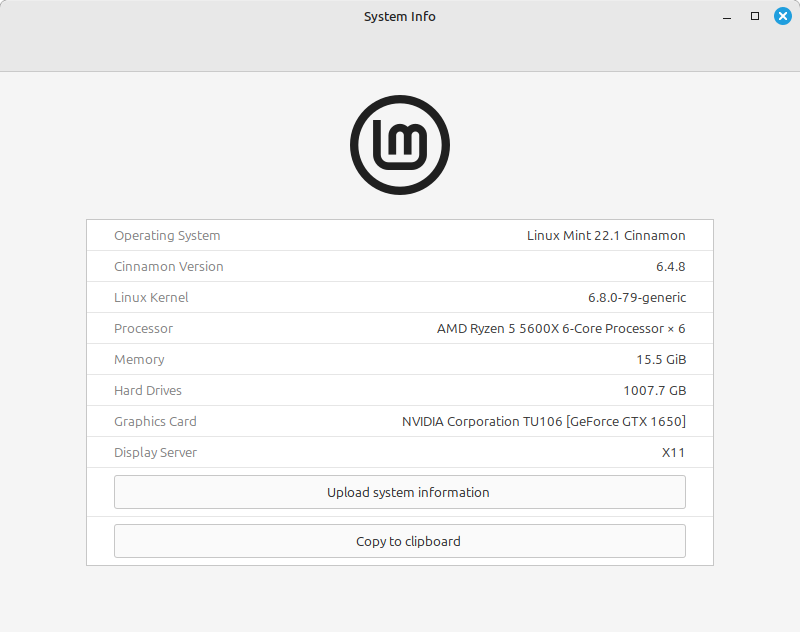
\includegraphics[width=0.85\textwidth]{resources/ej1a.png}
  \caption{System info}
\end{figure}

\subsection*{a- ¿Qué Sistema Operativo tiene instalado? ¿Qué distribución? ¿Qué versión?}
El sistema operativo que tengo instalado es Linux Mint 22.1 Cinnamon y es la version 6.4.8

\subsection*{b- ¿Cuántos procesadores posee su sistema de computadora? ¿Cuáles son sus características?}
En mi computadora tengo instalado un AMD Ryzen 5 5600X y cuenta con 12 procesadores(Hilos log)

\subsection*{c- ¿Cuál es la capacidad de memoria disponible?}

La memoria disponible es de \(15.5 GiB\).

\subsection*{d- ¿Qué placa de video o gráfica posee?}

La placa de vídeo es la GeForce GTX 1650 del fabricante NVIDIA.

\subsection*{e- ¿Cuál es la capacidad de disco que posee?}
La capacidad de disco con la que cuenta la computadora es de 1007.7Gb

%----------------------------------------------------------------------------------------

\section*{Ejercicio 2:}

\begin{figure}[h]
  \centering
  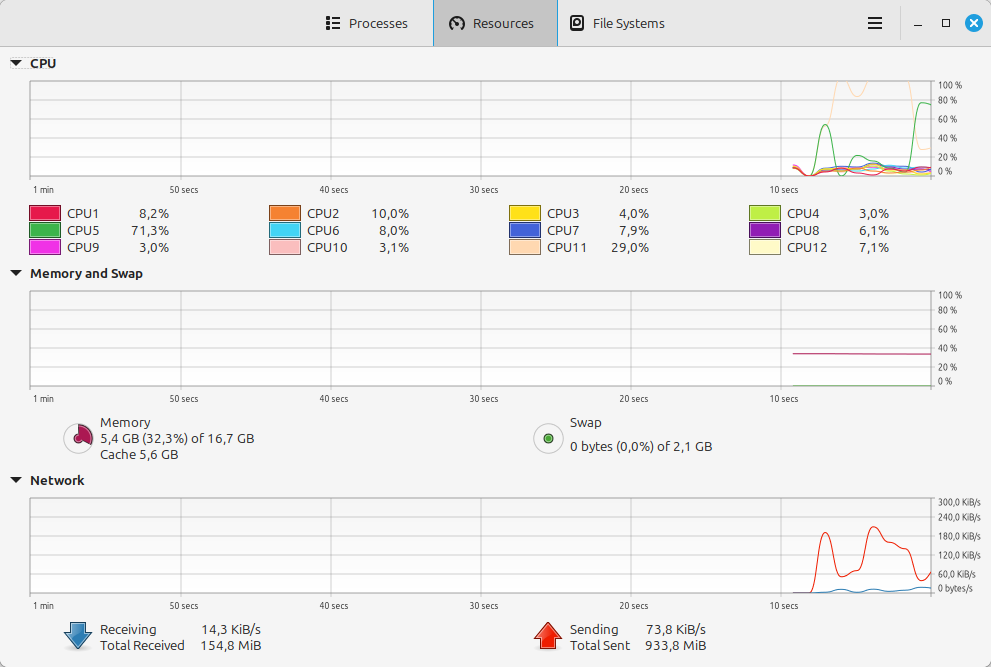
\includegraphics[width=0.85\textwidth]{resources/2.png}
  \caption{System monitor}
\end{figure}

\subsection*{a- ¿Qué información del sistema muestra?}

Al abrir el \textit{monitor de sistema} podemos observar:

\begin{itemize}
    \item \textbf{Uso de la CPU: } Muestra un histograma del uso de los procesador en tiempo real.
    \item \textbf{Uso de la memoria y espacio intercambiado (swap)\footnote{Herramienta de gestión de memoria que actua cuando la memoria RAM física se llena}: }
    Muestra de forma gráfica el uso de la memoria RAM y el espacio de intercambio.
    \item \textbf{Actividad de Red: } Muestra de manera gráfica la transmisión de  datos de red.
\end{itemize}

\subsection*{b- Mencione y describa qué información relevante sobre “Procesos” se puede mostrar (pestaña de “Procesos”).}

\begin{figure}[h]
  \centering
  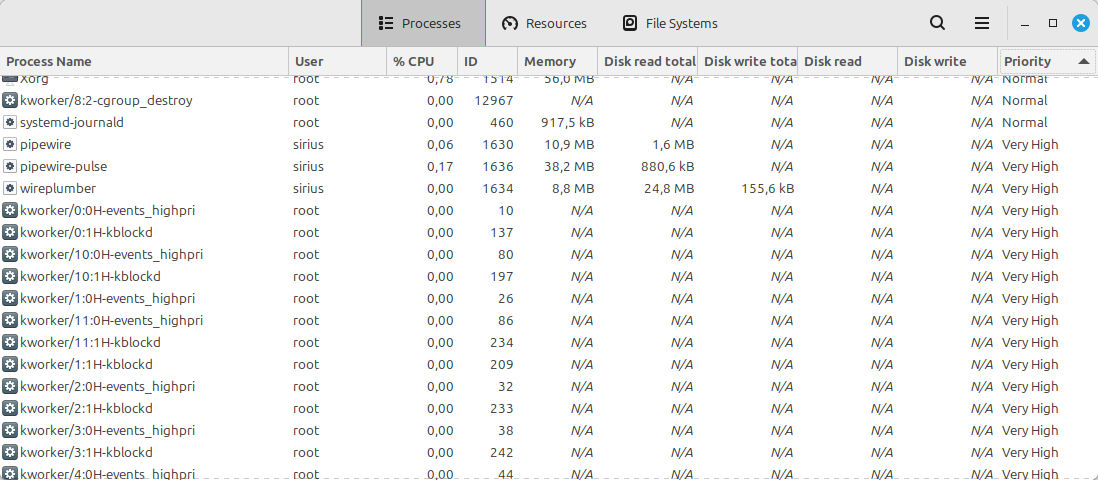
\includegraphics[width=0.85\textwidth]{resources/ej2b2.png}
  \caption{System monitor: Process}
\end{figure}

\begin{figure}[h]
  \centering
  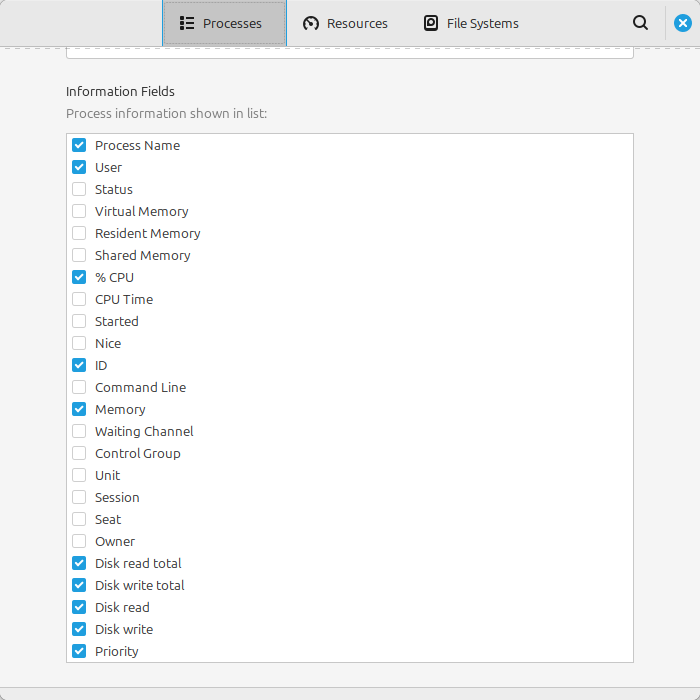
\includegraphics[width=0.5\textwidth]{resources/ej2b.png}
  \caption{System monitor: informacion de procesos}
\end{figure}

En dicha pestaña se muestra informacion en tiempo real de todos los procesos activos en el sistema. De ellos podemos ver:
\begin{itemize}
  \item \textbf{Nombre de Proceso: }Indica el programa que esta ejecutando
  \item \textbf{Usuario:} Indica que usuario inicio el proceso.
  \item \textbf{Uso de CPU:} Porcentaje del procesador que esta consumiendo el proceso
  \item \textbf{Id:} Numero unico que identifica a cada proceso
  \item \textbf{Memoria:} Cantidad de memoria RAM que esta consumiendo el proceso
  \item \textbf{Lectura de disco:} Cantidad de informacion leida desde el disco por el proceso
  \item \textbf{Escritura de disco:} Cantidad de informacion escrita en el disco por el proceso
  \item \textbf{Prioridad:} Indica que priorida le da el sistema al proceso frente a otros.
  \item \textbf{Estado:} Indica si el proceso esta durmiendo, ejecutandose,etc
\end{itemize}
  
\subsection*{c- ¿Qué operaciones se permite hacer respecto a los procesos?}
Las operaciones que se permiten hacer sobre un proceso son:
\begin{itemize}
  \item \textit{Open Files}
  \item \textit{Change Priority}
  \item \textit{Set Affinity}
  \item \textit{Stop}
  \item \textit{continue}
  \item \textit{Terminate}
  \item \textit{Memory Maps}
  \item \textit{Kill}
  \item \textit{End Procesos}
  \item \textit{Show Process Properties}
\end{itemize}

\subsection*{d- ¿Cómo se muestran las prioridades de un proceso?}

Las prioridades se muestran en una columna dedicada, donde cada proceso (fila) puede tomar los valores de: \textit{Very High}, \textit{High}, \textit{Normal}, 
\textit{Low}, \textit{Very Low}, \textit{Custom}

\subsection*{e- Inicializar las siguientes aplicaciones: un navegador Web, un procesador de texto y una
terminal/consola, luego responda observando la pestaña “Procesos” del Monitor de sistema:}

\begin{itemize}
    \item i- ¿Cuál es el ID (o PID, identificador del proceso) de cada proceso?
    \item ii- ¿En qué estado se encuentran cada uno de los procesos asociados a dichas aplicaciones?
    \item iii- ¿Qué proceso está en estado de ejecución?
    \item iv- Observar el tipo de cola (o Canal en espera) en la que puede estar un proceso según su
        estado.
    \item v- ¿Qué ocurre cuando se selecciona, para un proceso determinado, la opción de Detener,
        Finalizar o Matar un proceso? (presione botón derecho sobre un proceso elegido)
\end{itemize}

\begin{itemize}
  \item Brave web browser: Cuando se abre Brave muchos subprocesos de brave son abiertos (correspondiente a cada pestaña)
  \begin{itemize}
    \item ID 11249
    \item Estado: Alternan entre los procesos como running y sleeping, por lo que se encuentran algunos procesos en ejecución.
    \item Al detener el proceso se cierra completamente.
    \item Al matar el proceso también se cierra.
    \item El detener es similar.
  \end{itemize}
\end{itemize}
\begin{center}
    \begin{tabular}{|c|c|c|c|c|c|c|}   
    \hline
      \textbf{Proceso} & \textbf{ID} & \textbf{Estado} & \textbf{Ejecución?} & \textbf{Detención} & \textbf{Finalizar} & \textbf{Matar} \\
    \hline
      \textbf{Brave web browser} & 11249 & Running & Si & 34 & d & d\\
    \hline
  \end{tabular}
 \end{center}

 % \begin{center}
%     \begin{tabular}{|c|c|c|c|c|c|c|}   
%     \hline
%       \textbf{Proceso} & \textbf{ID} & \textbf{Estado} & \textbf{Ejecución?} & \textbf{Detención} & \textbf{Finalizar} & \textbf{Matar} \\
%     \hline
%       \textbf{Brave web browser} & 11249 & Running\footnote{En el momento de ejecutar Brave, se generan muchos procesos de Brave que intercalan entre running y sleeping} & Si & 34 & d & d\\

\subsection*{f- Desde la pestaña “Procesos”, ordene los procesos por número de proceso, donde se muestren los
siguientes datos (identificador del procesos, nombre del proceso, usuario, propietario, estado,
prioridad, memoria real):}

\begin{itemize}
    \item i. Muestre la información de los 10 primeros procesos (con captura de pantalla).
    \item ii. Complete la siguiente tabla de los procesos solicitados:
\end{itemize}

  Tabla de procesos de acuerdo al turnaround time
  \begin{center}
    \begin{tabular}{|c|c|c|c|c|}   
    \hline
      \textbf{Proceso} & \textbf{TT FIFO} & \textbf{TT SJF} & \textbf{TT Prio} & \textbf{TT RR} \\
    \hline
      \textbf{P1} & 10 & 34 & 22 & 34 \\
    \hline
  \end{tabular}
 \end{center}
%----------------------------------------------------------------------------------------

\section*{Ejercicio 3: Inicie el simulador Planificador de Procesos:}

\begin{itemize}
    \item En el sistema operativo Linux, descomprimir y abrir la carpeta del simulador.
    \item Una vez dentro de la carpeta del simulador “Planificador de Procesos”, abrir una “terminal o
consola” e ingresar: java VentanaPrincipal2
    \item Presione Enter para ejecutar el simulador.
    \item Lea el Manual de Ayuda del simulador
    \item Identifique los íconos del menú de herramientas, que representan las posibles operaciones del
simulador.
\end{itemize}

\begin{center}
    \begin{tabular}{|c|c|c|c|c|}   
    \hline
      \textbf{Proceso} & \textbf{TT FIFO} & \textbf{TT SJF} & \textbf{TT Prio} & \textbf{TT RR} \\
    \hline
      \textbf{P1} & 10 & 34 & 22 & 34 \\
    \hline
  \end{tabular}
 \end{center}


\subsection*{a- ¿Qué partes del diagrama del ciclo de vida de un proceso se pueden visualizar en la ventana
principal?}
\subsection*{b- ¿Qué información de los procesos puede ser visualizada? Ejemplifique.}
\subsection*{c- Respecto a la configuración de la simulación. ¿Qué información de los procesos se puede
configurar?}
\subsection*{d- ¿Qué información importante se puede observar una vez ejecutada la simulación?}
%----------------------------------------------------------------------------------------

\section*{Ejercicio 4: Inicialice la aplicación Terminal de Linux}


\subsection*{a- Utilizando el comando ps listar los procesos del sistema.}
\begin{figure}[h]
  \centering
  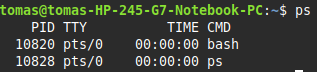
\includegraphics[width=0.85\textwidth]{resources/4a.png}
  \caption{System monitor: Process}
\end{figure}
\subsection*{b- Utilizando el comando ps con el parámetro -u listar los procesos del usuario actual únicamente.}
\begin{figure}[h]
  \centering
  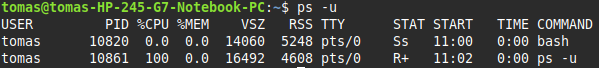
\includegraphics[width=0.85\textwidth]{resources/4b.png}
  \caption{System monitor: Process}
\end{figure}
\subsection*{c- Utilizando el comando top listar los procesos.}
\begin{figure}[h]
  \centering
  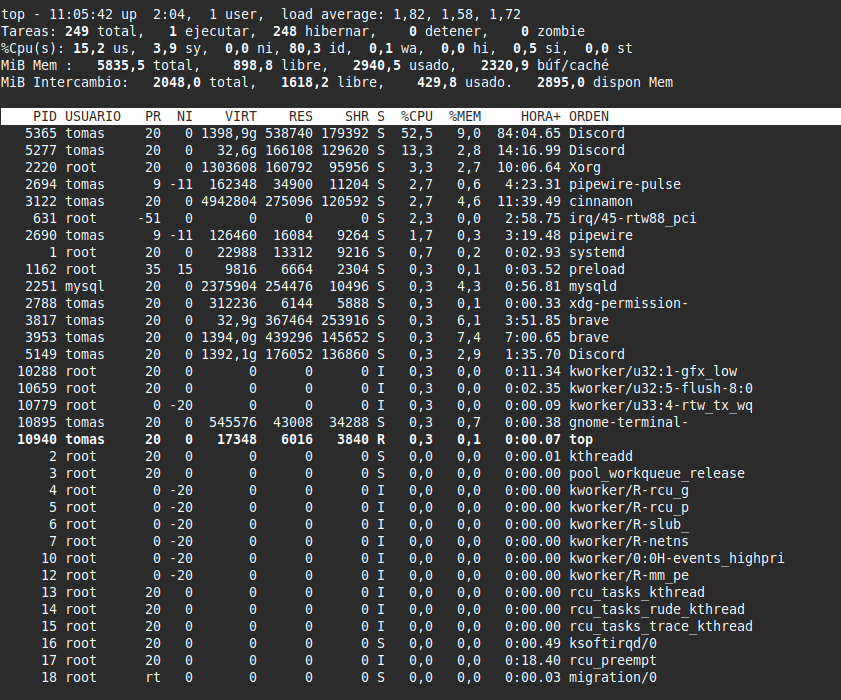
\includegraphics[width=0.85\textwidth]{resources/4c.png}
  \caption{System monitor: Process}
\end{figure}
\subsection*{d- ¿Cuál es la diferencia de utilizar el comando top respecto de utilizar el comando ps?}
El comando "ps" muestra el estado de los procesos de un momento determinado, es estático, es decir que no se actualiza automaticamente.
Por otra parte, el comando "top" muestra de manera interactiva y en tiempo real como cambia el estado de los procesos .
\subsection*{e- Observe la estructura jerárquica de los procesos en Linux utilizando el comando pstree.}
\begin{figure}[h]
  \centering
  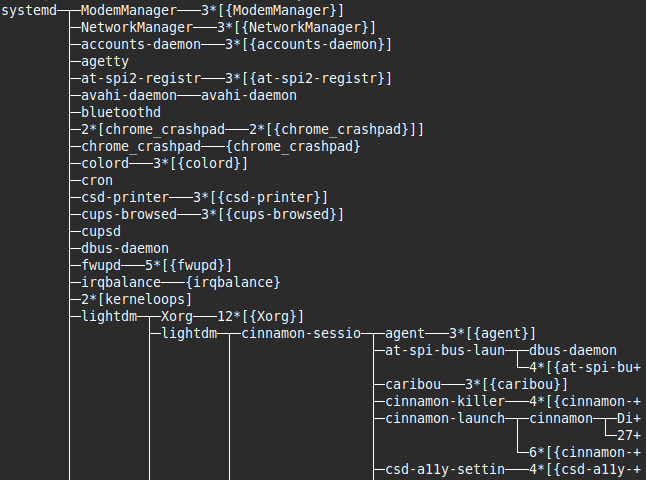
\includegraphics[width=0.85\textwidth]{resources/4e.png}
  \caption{System monitor: Process}
\end{figure}
Este comando muestra los procesos de manera que, indica cuales son "padres" y cuales "hijos".
"Systemd" es el primer proceso que ejecuta linux y este va ser el padre de casi todos los demas.
Podemos observar que algunos de sus hijos son "modem manager", "network manager", "accounts-daemon",etc
\subsection*{f- Ejecute el comando htop, luego visualice los estados de los procesos a través de la columna S (state).}
\begin{figure}[h]
  \centering
  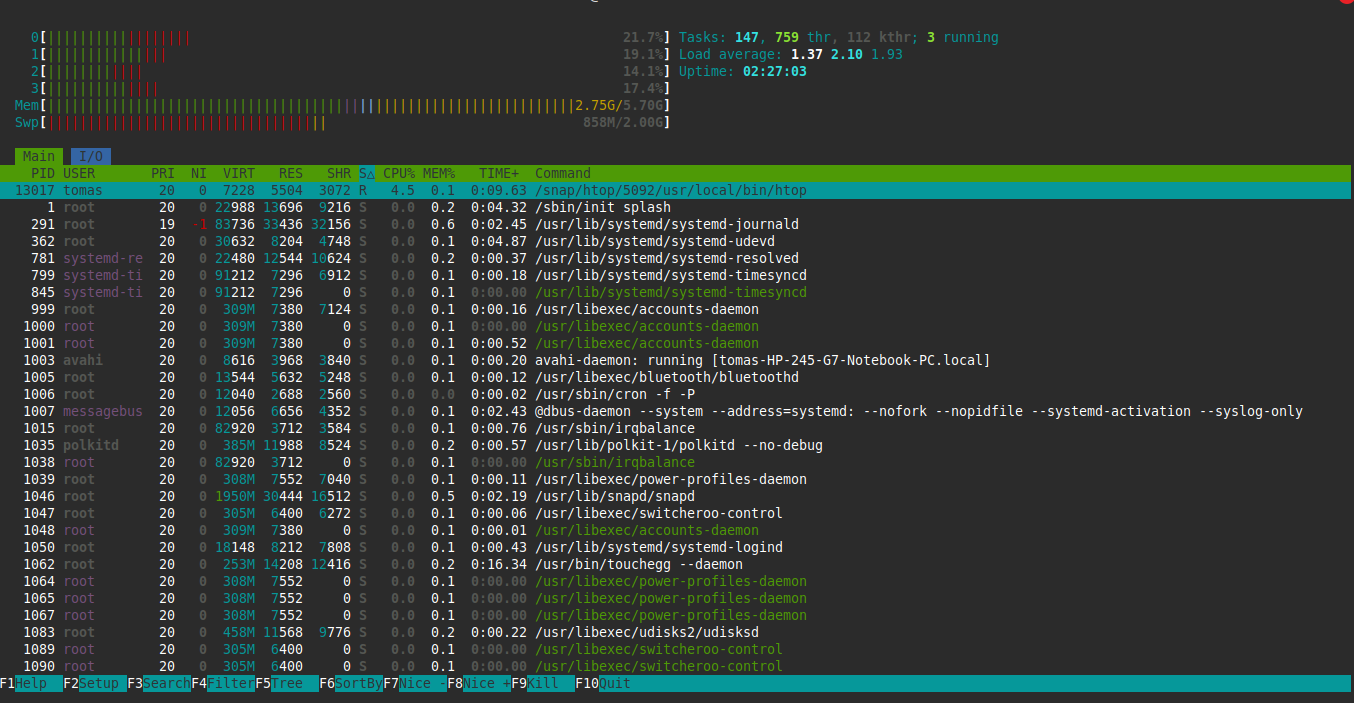
\includegraphics[width=0.85\textwidth]{resources/4f.png}
  \caption{System monitor: Process}
\end{figure}
La columna "S" que resulta del comando "htop" muestra el estado de un proceso.  
\subsection*{g- Utilizando el comando kill listar las opciones de parámetros posibles utilizando el parámetro -l, luego
investigue qué parámetros son necesarios para matar un proceso, muestre un ejemplo donde elige
un proceso para matar y luego lo mata aplicando el comando con los parámetros correspondiente.}
Listamos todas las señales posibles con el comando "kill -l"
\begin{figure}[h]
  \centering
  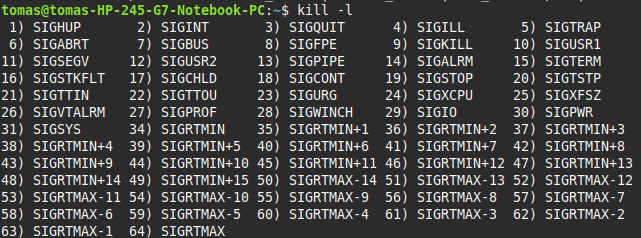
\includegraphics[width=0.85\textwidth]{resources/4g1.png}
  \caption{System monitor: Process}
\end{figure}
Cada número o nombre representa una señal que podés enviar a un proceso.
	Las más usadas para terminar procesos son:
	SIGTERM (15) → finalizar de manera ordenada
	SIGKILL (9) → matar forzadamente
  Existen ciertas diferencias entre ellas: 
    SIGTERM: Se le pide al proceso que termine dando la posibilidad de cerrar archivos, guardar datos,
    liberar memoria y limpiar recursos antes de salir. El proceso podria ignorar la señal y no termina.
    SIGKILL: Se le pide al proceso que termine de manera forzada u obligatoria y no le da posibilidad de cerrar archivos abiertos,
    liberar recursos ni tampoco de guardar. El proceso no puede ignorar esta señal

    Veamos un ejemplo de uso:
    Listamos los procesos usando el comando "top"
    \begin{figure}[h]
      \centering
      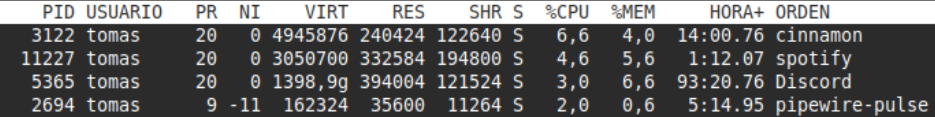
\includegraphics[width=0.85\textwidth]{resources/4g2.png}
      \caption{System monitor: Process}
    \end{figure}

    Voy a matar el proceso Discord el cual tiene como PID 5365
    Para finalizar amigablemente, usamos -SIGTERM ó -15 equivalentemente
    \begin{figure}[h]
      \centering
      
\includegraphics[width=0.85\textwidth]{resources/4g3.png}
      \caption{System monitor: Process}
    \end{figure}

    Si no se cierra procedemos a usar -9 o -SIGKILL
    \begin{figure}[h]
      \centering
      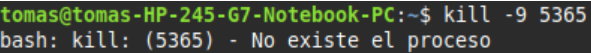
\includegraphics[width=0.85\textwidth]{resources/4g4.png}
      \caption{System monitor: Process}
    \end{figure}
    en este caso, el mensaje es que el proceso no existe porque fue eliminado anteriormente con "SIGTERM"

%----------------------------------------------------------------------------------------

\end{document}